\documentclass[a4paper]{report}

\usepackage{lipsum}
\usepackage{graphicx}

\usepackage{titling}
\newcommand{\subtitle}[1]{
  \posttitle{
    \par\end{center}
    \begin{center}\large#1\end{center}
    \vskip0.5em}
}

\title{\textbf{Foudi}}
\subtitle{Food order and delivery platform}
\author{Ali, Kadi, Hadj}
\date{\today}





\begin{document}
\maketitle

\chapter*{Remerciement}
\begin{center}
\Large \textbf{\textit{Tout d'abord, nous remercions Dieu, notre créateur, pour nous avoir donné la force, la volonté et le courage d'accomplir ce modeste travail.\\
Nous remercions notre directeur de thèse Monsieur Allaoui et Madame Kerrouche pour leurs conseils et leur encadrement du début à la fin de ce travail.\\
Nos remerciements vont à tous ceux qui ont contribué de près ou de loin à la réalisation de ce travail. Enfin, nous tenons à exprimer notre profonde gratitude à nos familles qui nous ont toujours soutenus et à tous ceux qui ont participé à la réalisation de cette thèse. Ainsi qu'à tous les enseignants qui ont contribué à notre formation.}}
\end{center}

\chapter*{Dédicaces}
\begin{center}
\Large \textbf{\textit{Nous dédions ce modeste ouvrage à nos parents bien-aimés qui nous ont soutenus tout au long de notre vie.\\
À nos amis qui n'ont jamais hésité à nous aider de quelque manière que ce soit.\\
Et à tous ceux qui nous ont enseigné tout au long de notre vie scolaire.\\
A nos camarades de la 3ème année LMD.\\
Merci à tous.}}
\end{center}

\newpage
\chapter*{Abstract}


\tableofcontents

\newpage
\chapter*{figure list}
\addcontentsline{toc}{chapter}{figure list}

\newpage
\chapter*{abbriviations}
\addcontentsline{toc}{chapter}{abbriviations}
	\begin{itemize}
		\item[\textbf{MVC}:] Model View Controller
		\item[\textbf{UI}:] User Interface
		\item[\textbf{SDK}:] Software Development Kit
		\item[\textbf{UML}:] Unified Modeling Language
		\item[\textbf{NoSQL}:] Not only Structured Query Language
		\item[\textbf{JSON}:] Java Script Object Notation
	\end{itemize}


\newpage
\chapter*{Introduction}
    Au cours de la dernière décennie, nous avons assisté à une révolution dans les commerces en ligne. Les gens se sont habitués aux achats en ligne et aux réservations à distance comme la réservation de billets, l'achat d'articles et même la commande de nourriture, principalement parce que c'est plus rapide, sans effort et moins compliqué.

Lorsque quelqu'un veut acheter de la nourriture en ligne, il doit vérifier un restaurant qui fabrique la nourriture qu'il veut, puis la nourriture doit lui être livrée soit par le livreur du restaurant, soit par un établissement de livraison séparé.

Comme nous l'avons vu dans les pays étrangers en Europe ou aux États-Unis, beaucoup de restaurants et de sociétés de livraison ont leur propre application mobile. Malheureusement, tous les établissements ne peuvent pas se permettre de créer leur propre application en raison des coûts élevés de développement d'une application mobile.

Notre solution est une plateforme conçue comme une application mobile qui regroupe les clients, les restaurants et les sociétés de livraison en un seul endroit. Elle répond à tous les besoins des personnes qui veulent commander leur nourriture à distance, elle permettra également aux propriétaires de restaurants et aux sociétés de livraison d'augmenter leurs ventes et d'accélérer leur flux de travail avec les clients à distance.

\addcontentsline{toc}{chapter}{Introduction}

\newpage
\chapter{theory}
	\section{Developement Android} Nous avons choisi de réaliser une application mobile dédiée aux utilisateurs d'Android, et nous avons beaucoup de choix quant aux technologies que nous allons utiliser pour le développement.
		\subsection{technologies used} Nous avons utilisé le framework Flutter pour les interfaces et la logique de l'application, et Cloud Firestore de Firebase pour le stockage et la gestion de la base de données.
		
			\subsubsection*{Flutter} Un kit de développement logiciel d'interface utilisateur open-source créé par Google. Il est utilisé pour développer des applications multiplateformes pour Android, iOS, Linux, Mac, Windows, et le Web à partir d'une base de code unique.
Nous avons utilisé Flutter en raison de sa structure qui favorise la vitesse de développement. Sa structure est simplement une cascade de widgets faciles à personnaliser.

Flutter utilise le langage de programmation Dart, également développé par Google. Il s'agit d'un langage orienté objet, basé sur des classes, avec une syntaxe de type de la language C.
			\subsubsection*{Firebase} la plateforme mobile de Google qui aide à développer rapidement des applications de qualité. Elle dispose de nombreuses fonctionnalités, mais nous l'utilisons principalement pour son service de stockage au Cloud (Cloud Firestore).
				\paragraph*{Cloud Firestore} est une base de données documentaire NoSQL (un ensemble de continuation en cascade collection-document) qui nous permet de stocker, de synchroniser et d'interroger facilement des données pour des applications mobiles et web - à l'échelle mondiale.
	\section{collab working method}
		Cette application a été développée à partir de zéro par trois développeurs, nous devions travailler en parallèle sur le même projet, nous avons donc utilisé Git et Github.

		\subsection*{Git} C'est un logiciel permettant de suivre les modifications apportées à un ensemble de fichiers. Il est généralement utilisé pour coordonner le travail des programmeurs qui collaborent à l'élaboration du code source lors du développement de logiciels. Ses objectifs sont la rapidité, l'intégrité des données et la prise en charge des flux de travail distribués et non linéaires.

		\subsection*{Github} C'est un service d'hébergement de référentiel Git, mais il ajoute de nombreuses fonctionnalités qui lui sont propres. Il fournit une interface graphique basée sur le Web. Il fournit également un contrôle d'accès et plusieurs fonctions de collaboration.
	\section{architecture} %include the sequence chart of flutter in mvc
		Nous avons utilisé l'architecture de projet MVC. Il s'agit d'un modèle de conception de logiciel couramment utilisé pour développer des interfaces utilisateur qui divisent la logique du programme en trois éléments interconnectés.

Cela permet de séparer les représentations internes de l'information de la manière dont l'information est présentée à l'utilisateur et acceptée par celui-ci.
\begin{figure}[!h]
  \center
  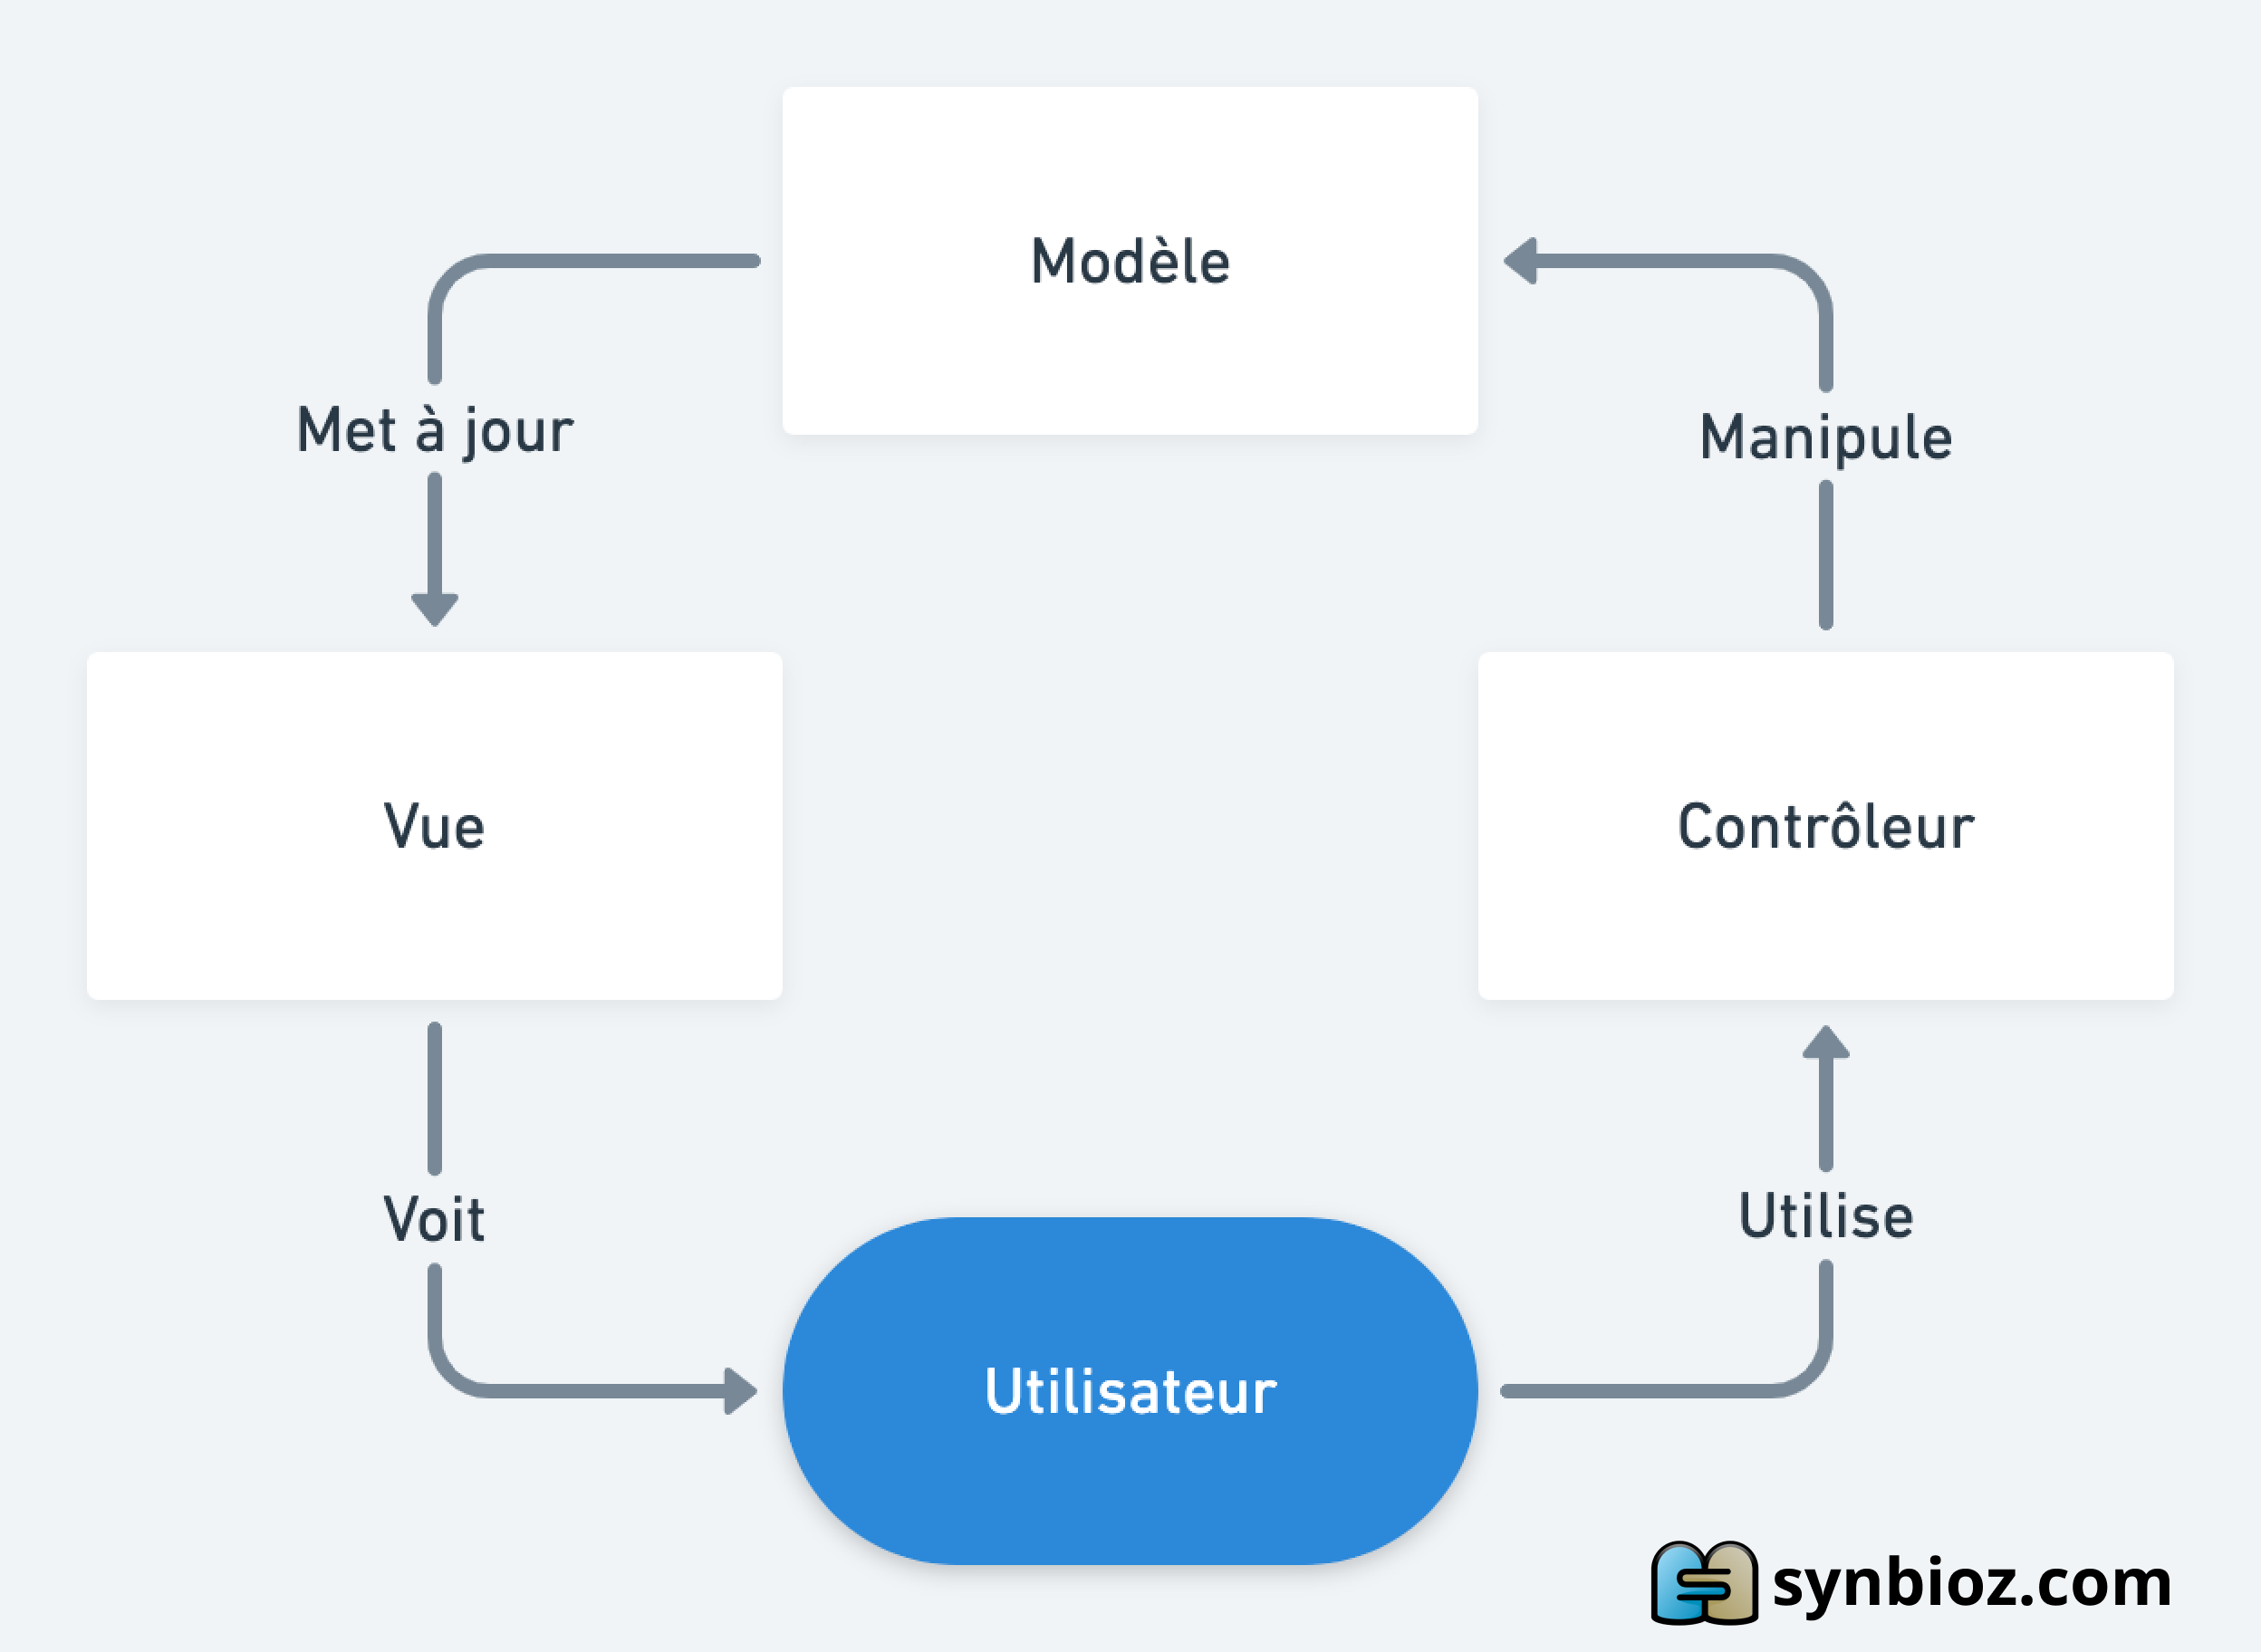
\includegraphics[width=10cm]{mvc.png}
  \caption{Le flux MVC}
  \label{fig:fluxmvc}
\end{figure}

\newpage
\chapter{Conception}
	\section{Modelisation} UML diagrammes
		\subsubsection{Diagramme des classes} image + brief explanation
		\subsubsection{Diagramme des cas}
		\subsubsection{Diagramme de sequences}
	\section{Code structure}
		\subsection{models} %listing
			bla bla and then listitems with description if needed
			\subsubsection{JSON parsing}
		\subsection{controllers}
		\subsection{views}
		small description on what are views and how are they used and implemented
		\subsection{widgets}
		
\newpage
\chapter{Realisation}
	\section{Startup} sign in and up
	\section{Client case} flows
	\section{Restaurant case} flows
	\section{Deliverer case} flows

\newpage
\chapter*{Conclusion}
blblabla
\addcontentsline{toc}{chapter}{Conclusion}

\newpage
\begin{thebibliography}{300}
\end{thebibliography}

\end{document}
